\documentclass[twocolumn]{article}
% {amsart}
\usepackage[top=0.75in, left=0.65in, right=0.65in, bottom=0.6in]{geometry}

\usepackage{float}

% \usepackage{url}
% \usepackage{xurl}
\usepackage[pdftex]{hyperref}


% \usepackage{code}
% \usepackage{cite}
\usepackage{latexsym}
\usepackage{amsmath}
\usepackage{amssymb}
\usepackage{graphicx}
% IPA symbols. safe turns off overrides for like \! which I still want
\usepackage[safe]{tipa}
\usepackage{chessboard}
% \usepackage{chessfs}
% \usepackage{adjustbox}

\usepackage[most]{tcolorbox}

% lets me explicitly set a. or 1. etc. as enum label
% \usepackage{enumitem}

\pagestyle{empty}

\usepackage{ulem}
% go back to italics for emphasis, though
\normalem

\usepackage{natbib}

\interfootnotelinepenalty=0
\setlength{\footnotesep}{2em}

\newcommand\sfrac[2]{\!{}\,^{#1}\!/{}\!_{#2}}

% XXX the collection of crap above causes a first page
% with just "1" on it (probably conflicting packages). This
% magic just drops the first page, which is of course not
% the right solution, but...
\usepackage{atbegshi}% http://ctan.org/pkg/atbegshi
\AtBeginDocument{\AtBeginShipoutNext{\AtBeginShipoutDiscard}}

\newcommand\upsigbovik{
  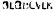
\includegraphics[height=1em]{upsigbovik}
}

\begin{document}

\title{Lowestcase and Uppestcase letters: Advances in Derp Learning}
\author{Dr.~Tom~Murphy~VII~Ph.D.}\thanks{
Copyright \copyright\ 2021 the Regents of the Wikiplia Foundation.
Appears in \upsigbovik~2021 with the
OS2TypoLinegap of the Association for Computational Heresy; {\em IEEEEEE!}
press, Verlag-Verlag volume no.~0x40-2A. 1 em}

\setchessboard{showmover=false}

\newcommand\makelowercase{{\sf make\_lowercase}}
\newcommand\makeuppercase{{\sf make\_uppercase}}

\renewcommand\th{\ensuremath{{}^{\textrm{th}}}}
\newcommand\st{\ensuremath{{}^{\textrm{st}}}}
\newcommand\rd{\ensuremath{{}^{\textrm{rd}}}}
\newcommand\nd{\ensuremath{{}^{\textrm{nd}}}}
\newcommand\at{\ensuremath{\scriptstyle @}}

\renewcommand\paragraph[1]{\smallskip \noindent{\bf #1}\enspace}

\date{1 April 2021}

\maketitle \thispagestyle{empty}

\sloppypar


\section{Introduction}

Have you ever been writing something on the internet and wanted to convey
that you ARE FEELING ANGRY? Conversely, have you ever fired back a super
quick dm and u wanted to make it clear that it was like super ca\textipa{Z}
and so u didnt use ne capitals or punctuation dots except 4 that one place
where u needed to use the international phonetic alphabet because u dont
no how to write ca\textipa{Z} as in short for casual without it lol

If so, you made use of the fact that all letters have UPPERCASE
VERSIONS (e.g.~signifying ANGER) and lowercase versions
(e.g.~signifying u dont care lol). These dimensions have other uses,
for example, it is polite to start a person's name with a capital
letter to show that you took the time to regard their humanity (as it
takes extra work to press the caps lock key, press the first letter of
their name, and then press the caps lock key again to turn it off).
In German, Nouns start with uppercase Letters, signifying Superiority
over other grammatical Categories like Verbs and Adjectives. Lowercase
letters can be used to conserve printer ink. Actually, I'm not sure that
lowercase letters have any other uses, but let's just roll with it.

The thing is: What if I'm even MORE ANGRY THAN I WAS BEFORE? There are
some standard sorts of typographic emphasis, like I can be {\bf BOLD
  ANGRY} or \textbf{\textit{\large BIG BOLD ITALIC UNDERLINE ANGRY}}
or { \Large \textbf{\textit{\uuline{COMBINE A LOT OF THESE ANGERS}}}},
each with its own nuances, depending on the cascading style sheet or
LaTeX class file. To be even more casual than lowercase, u can learn 2
write like this, and {\scriptsize shrink away} and also \sout{cross
  out ur words in shame in advance of them even being read}, but there
are few other options for de-emphasis. Plus, when I'm FEELING PRETTY
ANGRY, TOM, how do I capitalize that already-capitalized T in order to
show the proper reverence for your humanity?

This paper is about unshackling this dimension of human expression by
introducing letterforms further along the uppercase and lowercase
dimensions. Basically, we want to know what the upper{\it er}case
version of uppercase T is, and a lower{\it er}case version of
lowercase t is.

% shift-reduce conflict
% Shift is often used to increase conflict, not reduce it

\subsection{Induction}

Today we're just concerned with English letters, of which there are
only 26. To create an upperercase and lowerercase alphabet by hand is
O(52 pick up), which for a guy who likes drawing letters anyway and
who alphabetized Star~Wars for fun, is not much to ask. In fact I
drew such alphabets in Figure~\ref{fig:manual} just now.

\begin{figure}[ht]
% \includegraphics[width=0.9 \linewidth]{manual}
\caption{TODO} \label{fig:manual}
\end{figure}

But, why do easy fun things by hand when you can build a complicated
automatic solution which produces much worse results? Well, there is
no good reason. I could claim that this allows us to automatically
upperercase any font, which is true, but the results are at best
moderately letter-like lumps. In principle there are several other
interesting things we can do, like apply the function over and over to
approach the uppestcase and lowestcase letters. This sounds fun, but
the results themselves are not going to impress. But the story of
getting there may be interesting, and even as it turns out to be
``derp learning,'' there will be opportunities for more good puns. So
let's just roll with it!


\section{Capital A Artificial Intelligence}

% XXX introduce the meaning of the \letterform syntax somewhere?

\newcommand\letterform[1]{\tcbox[
    nobeforeafter,
    tcbox raise base,
    top=0pt,bottom=0pt,left=-1pt,right=-1pt,
    left skip=1pt,
    right skip=1pt,
    arc=2pt,outer arc=2pt,
    boxrule=0.15mm,
    colback=white,
    colframe=white!50!black
    ]{\textrm{#1}}}

We want to machine-learn~\cite{neuralnetwork} two functions,
\makelowercase\ and \makeuppercase. Each takes a letterform and
returns a letterform (we can choose how these are represented) and
does the needful, e.g.~\makelowercase(\letterform{A}) should return
\letterform{a}. In order to learn this function, we'll at least need a
lot of examples to use as training data. A training example for
\makelowercase\ is a letterform and its expected corresponding
lowercase one. We can ``easily'' find a large amount of examples by
using existing fonts, and pairing their \letterform{A} with their
\letterform{a}, and so on for all 26 letters, and symmetrically for
\makeuppercase.

However, if we only give uppercase letters to \makelowercase, it
may very well learn how to generate the corresponding lowercase letter
but be unable to do anything interesting for other letterforms. This
is a problem because we want to use this function to see
what e.g.~\makelowercase(\letterform{a}) is.

This is not (only) the problem of overfitting. An overfit model could
work well on the letter \letterform{A} from one font (because it has
seen that font before) but fail on \letterform{A} from a new font. The
property that we want is that the learned function can also produce an
interesting result on a shape it's never seen before, like
\letterform{\textipa{Z}}\,. That is, it has generalized the idea of
``how to make a shape lowercase,'' not simply ``how to make a capital
A shape lowercase.''

The problem with this is that we don't have any training data other
than existing fonts to tell us what the lowercase of some arbitrary
shape should look like. Without examples of this form, the problem is
unconstrained. \makelowercase\ could learn to generate empty output
for anything it doesn't recognize as a capital letter, and still have
perfect performance on the training and test set. It is hard to
generate training data of this form (even by hand) as we don't have
much idea {\em a priori} of what a lowerercase \letterform{a} should
look like (except for e.g.~One Artist's Impression from
Figure~\ref{fig:manual}).

\newcommand\trainingexample[2]{$\langle$\letterform{#1}$,\,$\letterform{#2}$\rangle$}

\newcommand\weirdcharlo{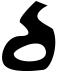
\includegraphics[width=0.75em]{weirdchar-lo}}
\newcommand\weirdcharup{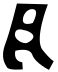
\includegraphics[width=0.75em]{weirdchar-up}}
\newcommand\lowerlowera{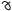
\includegraphics[width=0.6em]{lowerlowera}}

This brings us to the one decent idea in this paper (which by the way
only sort of works, but let's just roll with it). We can at least
express one characteristic property of the \makelowercase\ function
that ought to be true even for letterforms we don't have examples of:
It ought to be the inverse of \makeuppercase. So, we train these two
models in tandem. \makelowercase\ is fed training examples from the
sample fonts like \trainingexample{Q}{q} etc.~and \makeuppercase\ gets
\trainingexample{e}{E} etc.~as expected. We also run the current
version of \makeuppercase\ on some letter-like shapes, which produces
some other shape. For example, say that
\makeuppercase(\letterform{\weirdcharlo}) outputs
\letterform{\weirdcharup}. We have no idea if this is good or not, so
we don't update the model. However, we {\em do} provide the training
example to \trainingexample{\weirdcharup}{\weirdcharlo} to the
\makelowercase\ training queue and penalize {\em it} if it did not
predict \letterform{\weirdcharup}. In this way, whatever \makeuppercase\ is
doing, we ask \makelowercase\ to learn the inverse. We of course also
simultaneously do the symmetric thing, using the output of
\makelowercase\ to create training examples for
\makeuppercase\ (Figure~\ref{fig:cotraining}).



\begin{figure}[ht]
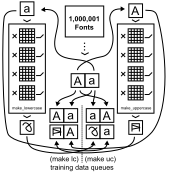
\includegraphics[width=0.9 \linewidth]{training}
\caption{ Simultaneously training the two models. This example
  illustrates how a pair of letterforms \letterform{A} and
  \letterform{a} from the same font becomes four training examples.
  The pair straightforwardly generates an example
  \trainingexample{A}{a} for the \makelowercase\ queue, and an example
  \trainingexample{a}{A} for the \makeuppercase\ queue. Separately, we
  supply \letterform{a} to the \makelowercase\ model, simply to get
  the current output \letterform{\lowerlowera} (no model updates are
  performed). But this pair reversed becomes a training example
  \trainingexample{\lowerlowera}{a} for the \makeuppercase\ queue.
} \label{fig:cotraining}
\end{figure}

Because \makelowercase\ is getting training examples of
uppercase/lowercase pairs from real fonts, it remains grounded on real
letters. It is also free to generate new shapes for the open domain
(outside \letterform{A}--\letterform{Z}). However, it is penalized if
its behavior is not the inverse of whatever \makeuppercase\ is
currently doing. And since we do the symmetric thing for
\makeuppercase\, there is a (slow) feedback loop between the two
models that keeps them from straying too far from the grounded
examples. The idea is that this allows them to do some creative
generalization outside their native domains, but in a way that
still has some constraint.

In practice, we don't feed arbitrary shapes to the models. We just
need something letter-like, and in fact we have a large collection of
letter-like shapes among our existing fonts! We pass already-lowercase
shapes to \makelowercase, in order to generate inversion examples for
training \makeuppercase. These shapes are clearly letter-like (they
{\em are} letters) and are also of interest to us anyway, since we
want to try to generate lowerercase and upperercase letters from
the trained models.


\section{1000001 Free Fonts}

% no copyright intended

Sprechen of Fonts, I downloaded every font I could find on the whole
internet. This was overkill. The resulting directory tree contained
over 100,000 files, many of which were duplicates. Exact duplicates
are easy to find, but since many of these files were the result of 30
years of community transmission, they had acquired various mutations.
One of the first things I did was write software to automatically
remove files that were essentially duplicates even if they weren't
exactly the same bytes.

Next, my lord, do people have bad taste! And I say this as someone who
made dozens of amateurish fonts~\cite{dbzfonts} as a high school and
college student and who is contributing several new questionable
fonts\label{sec:newfonts} as a result of this paper. The database is
just filled with garbage that is unusable for this project: Fonts that
are completely illegible, fonts that are missing most of their
characters, fonts with millions of control points, Comic Sans MS,
fonts where every glyph is a drawing of a train, fonts where
everything is fine except that just the lowercase r has a width of
{\tt MAX\_INT}, and so on. So I built a UI
(Figure~\ref{fig:sortition}) for efficiently and mind-numbingly
cleaning up the database by marking fonts as broken or suitable (and
also categorizing them as serif, sans-serif, decorative, techno, etc.,
which classifications I never used). In doing this I noticed another
extremely common problem, which was that many fonts had the same
letter shapes for uppercase and lowercase letters. This would not do
for the current application!

\begin{figure}[tp]
\centering
  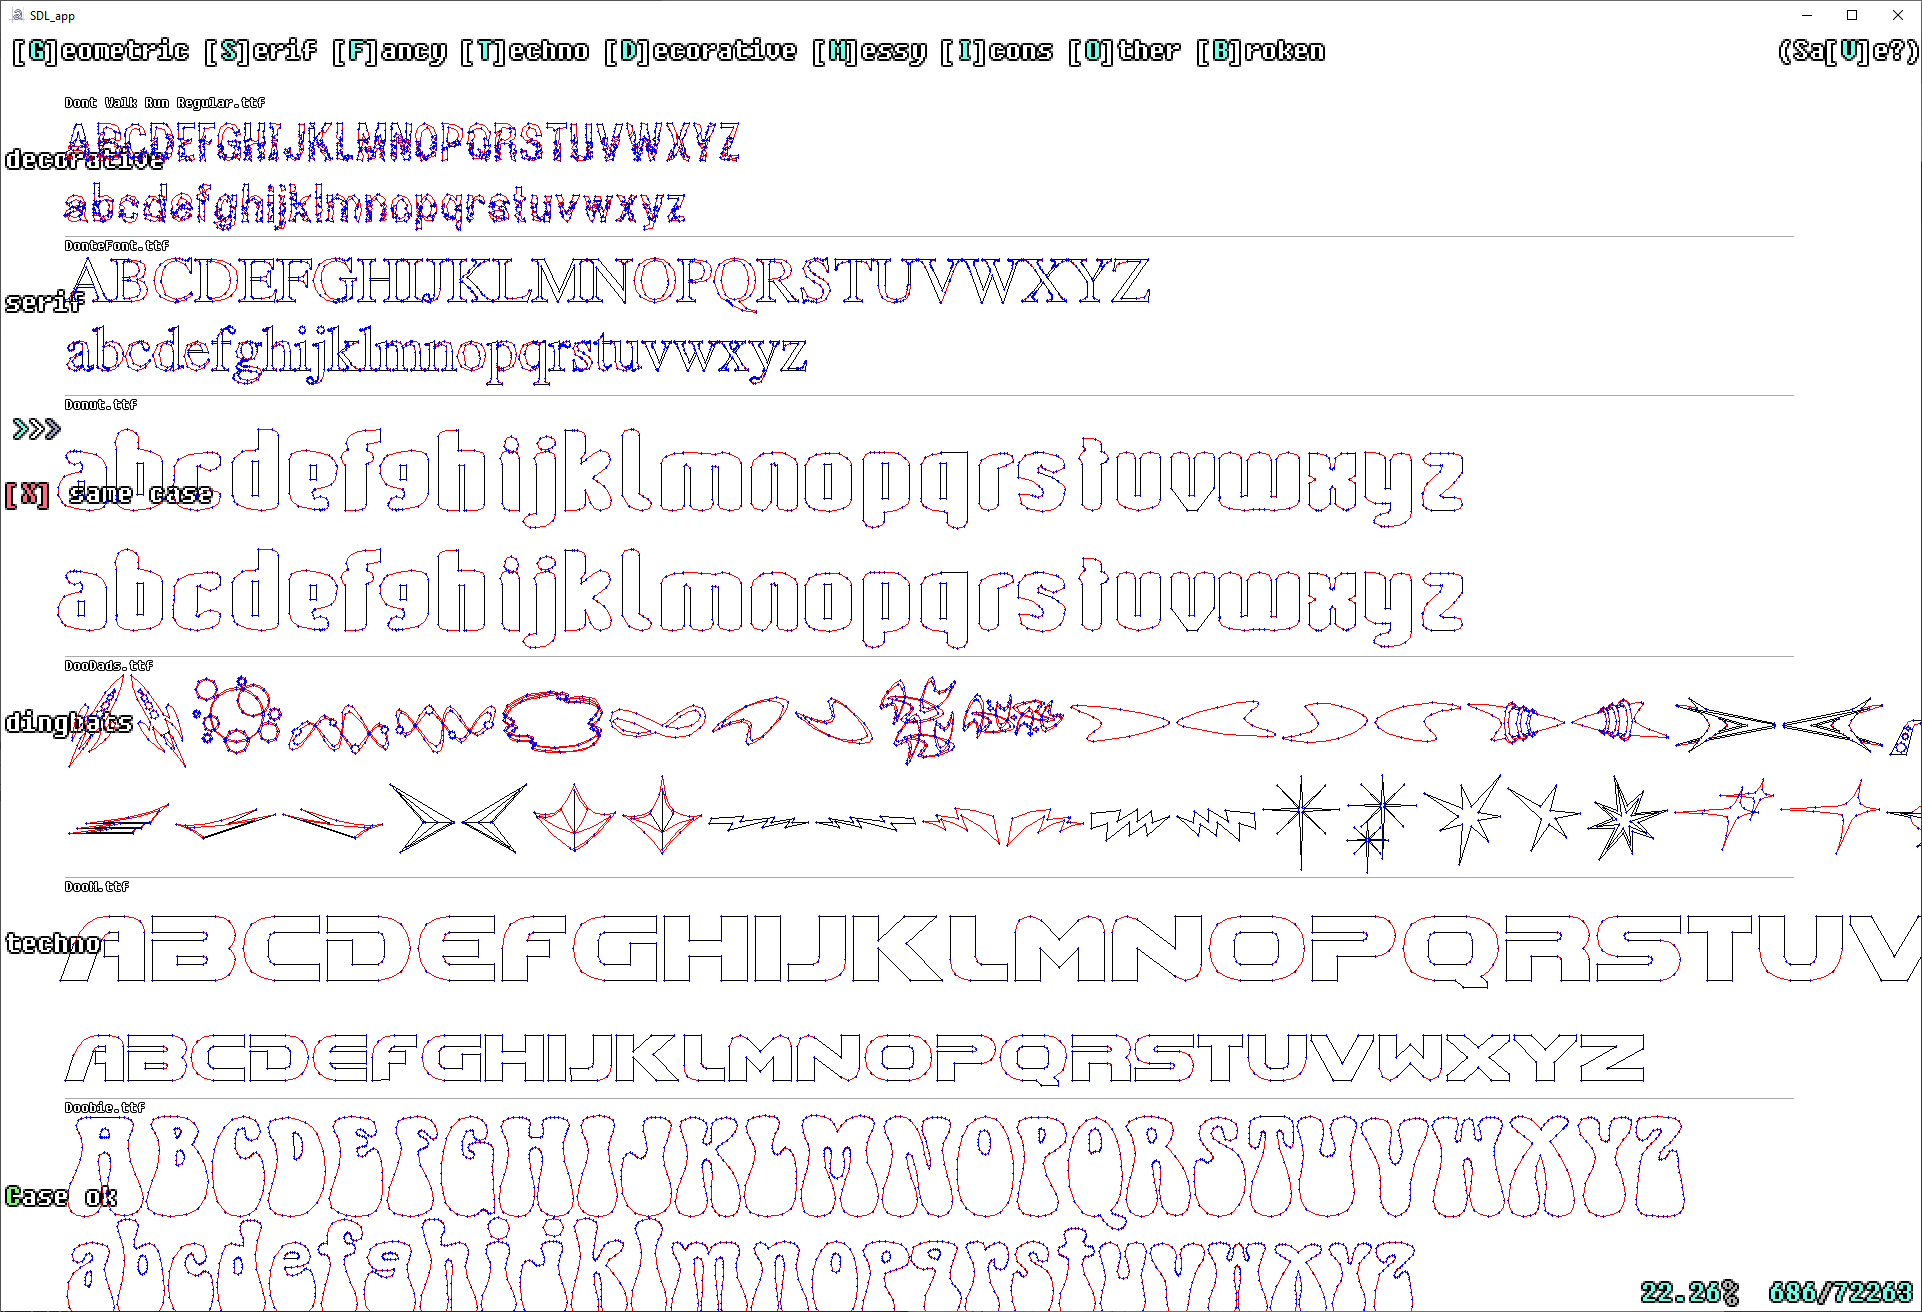
\includegraphics[width=0.98 \linewidth]{sortition}
\caption{ The interactive font data-cleaning UI. A seemingly endless
  series of fonts presents, with single keypresses putting the fonts
  into common categories such as (b)roken.
  % XXX maybe write more?
} \label{fig:sortition}
\end{figure}

But why manually mark fonts with nearly the same upper- and
lowercase letters, when you could build a complicated automatic
solution? The first pass identified fonts whose letters were
exactly the same, but this was only a small fraction of the
problematic fonts. A common issue was that the lowercase characters
were very slightly modified versions of the uppercase ones, often
scaled and translated and then perhaps ``optimized'' during the
font export.

So, for a given font, I want to reject it if for most pairs of cased
letters \letterform{A},\letterform{a}, \letterform{a} is close to a
linear transformation of \letterform{A}. This problem can probably be
solved with math, but it didn't sound that fun. Instead I tried out
a new tool, and it worked well enough that I've now added it to the
permanent rotation: Black-box function optimizers.

\paragraph{Black-box optimization.} If you have a function and want
to find arguments that minimize its output, the most efficient
techniques are generally those like gradient descent. (In fact, the
backpropagation algorithm we use to train the neural network in
Section~\ref{sec:neural} is gradient descent on the function that
takes the model weights and produces an error value for each output
node.) The problem with this is that you need to do some math to
compute the derivative of the function, and anyway you need to deal
with fiddly bits (Section~\ref{sec:fiddly}) unless the function is
convex and smooth, which it will not be. If you don't want to deal
with that, and have a fast computer (and who doesn't?), black-box
optimization algorithms are worth considering. Here, the
interface\footnote{ Here a simplfied wrapper around
  BiteOpt~\cite{biteopt} in my {\tt cc-lib} library. See
  \url{https://sourceforge.net/p/tom7misc/svn/HEAD/tree/trunk/cc-lib/opt/}.}
is just something like (C++):

\begin{verbatim}
  double Minimize1D(
      const std::function<double(double)> &f,
      double lower_bound,
      double upper_bound,
      int iters);
\end{verbatim}

which takes a function \verb+f+ of type \verb+double+ $\rightarrow$
\verb+double+, finite bounds on the argument's value, the maximum
number of times to call that function, and returns the argument it
found that produced the minimal value. Not as fast as gradient
descent, but in practice ``if the function is kinda smooth'' these
optimizers produce excellent results! The chief selling point for me
is that I don't need to think about anything except for writing the
function that I want minimized, which I just express in normal code.

\begin{figure}[tp]
\centering
  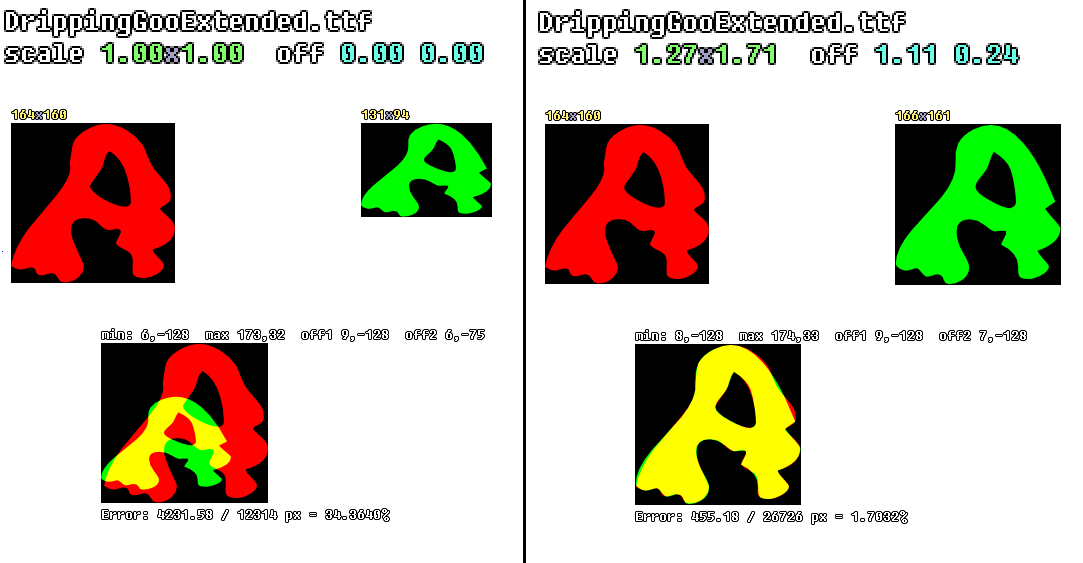
\includegraphics[width=0.9 \linewidth]{casealignment}
\caption{ Example alignment to reject the font {\tt
    DrippingGooExtended}. At left, \letterform{A} (red) and
  \letterform{a} (green) rendered with the identity transform, and
  their alignment ($35\%$ difference) below. At right, the transform
  found by the black-box optimizer and the resulting alignment with
  $1.7\%$ difference. Note that the shapes are still not an exact
  match (probably noise introduced in the font export process, which
  has to round the data to integers and might apply other non-linear
  transformations like curve simplification), but these are clearly
  not a useful pair for the current
  problem.} \label{fig:casealignment}
\end{figure}

In this case, I render the letterform \letterform{A} and then optimize
a four argument function taking {\tt xoff}, {\tt yoff}, {\tt xscale},
{\tt yscale}. This function renders \letterform{a} with those
parameters, then just computes the difference in the two rendered
bitmaps. This finds the best alignment of the two letterforms (under
the linear transformation) in a few hundred milliseconds
(Figure~\ref{fig:casealignment}). If the disagreement is low as a
function of the total pixels, then we say that the letters have the
same case. If enough of them have the same case, we reject the font. I
set the thresholds by looking at the P/R curve computed on random
hand-labeled examples (Figure~\ref{fig:samecasepr}).

\begin{figure}[ht]
\centering
  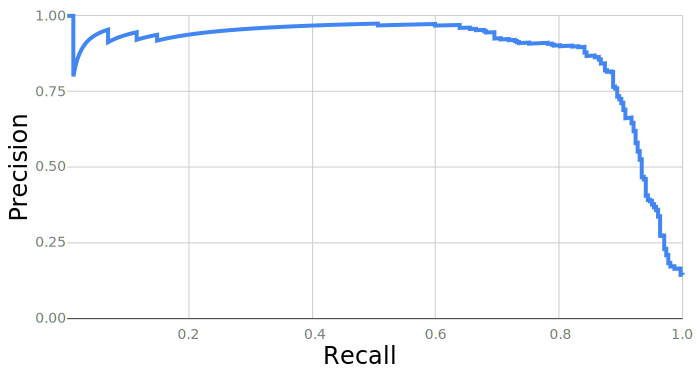
\includegraphics[width=0.9 \linewidth]{samecasepr}
\caption{ Precision--recall curve for automatically detecting fonts
  that have basically the same upper- and lowercase shapes. It's good!
  This is how you want 'em to look!
} \label{fig:samecasepr}
\end{figure}

\medskip

I labeled fonts using the UI until I had 10,000 that were clean enough
for a training set and passed the same-case heuristic.

\section{The simplest thing that might work} \label{sec:vectorversion}

Before getting fancy (which we we will) it's good engineering hygiene
to try the simplest thing that might just work (it doesn't). Fonts
are represented as vector data (lines and quadratic B\'ezier curves).
Can we just train a network that takes these lines and curves as input
and predicts the lower- or uppercased letter in the same format? (No.)

We'll at least put the data in a somewhat normalized form. The neural
network will take a fixed number of inputs to a fixed number of
outputs, so a simple approach is to decide on some maximum number
control points per letter, and only try training on fonts whose
letterforms fit within that budget. Letterforms can be made of
multiple contours (e.g.~a stacked \letterform{g} typically has two
holes in it, and \letterform{j} has two disjoint parts). I found that
most clean fonts had three or fewer contours, and when sorting them by
descending length, basically all of them fit within 100, 25, and 16
endpoints for the three. So, I only train on fonts where all of the
letters fit within this budget.\footnote{It would not be a good idea
  to reject only the letters that don't fit, because it might result
  in the network being trained on more \letterform{l}s (tends to be
  simple) than \letterform{g}s (tends to be complex).}

% TODO: Illustrate a letterform and its contours?

Rather than try to work with both lines and B\'ezier curves, I
normalize each contour to only contain B\'eziers, by turning a line
segment into an equivalent B\'ezier with its control point at the
midpoint. This frees us from having to distinguish the two types in
the data. We also need each of the three contours to not be {\em too
  short}, so I fill out the fixed-size buffers by repeating the last
point. This is not great but does have the correct meaning (bunch of
useless zero-length edges). It has the property that any predicted
data can be rendered and has a straightforward point-by-point error
function (which might not be the case if we were predicting a dynamic
number of points).

The network I trained has an input layer size of $570 = (100 + 25 + 16)
\times 4 + 3 \times 2$ (one control point and one end point per
B\'ezier curve), plus a starting point for each of the three contours.
The output layer is the same size, plus 26 (see below). There are
three hidden layers of size 308, 308, 360. The first layer is dense
and the remainder are sparse,
%(two thirds to a half of the weights are zero),
for just about 1 million total parameters. All layers are leaky
rectified linear units ({\tt x > 0 ? x : 0.1 * x}), which is fast to
compute and better than sigmoids in the output since correct values
will not just be 0 and 1. If you're taking notes, don't, as again this
does not work well, and I don't know how people figure out what the
right network size is anyway. I just made it up. You can give {\em me}
your notes.

\paragraph{Bonus outputs.} The output includes the predicted shape,
and also 26 individual predictors for each of the 26 letters. So a
training example is actually like \letterform{C} $\rightarrow$
\letterform{c} $[0, 0, 1, 0, 0, \ldots, 0]$, with the 1 in the third
place because C is the third letter. We don't need these outputs for
the problem itself (e.g.~to lowercase new letter shapes), but there
are several ideas behind this. First, the lowercasing function we're
trying to learn does depend on the letter of the alphabet being
lowercased (in an extreme case, consider the lowercase-L
\letterform{l} and the uppercase-i \letterform{I}, which look the same
in many fonts but have different lowercase letterforms). By asking the
network to learn this as well (it is penalized when it gets the
prediction wrong), it must learn features that allow it to distinguish
different letters, and those features are available for use by outputs
we {\em do} care about. This is an easy way to coax it to learn
features that I know are meaningful without having to actually
engineer feature extractors by hand (or first train separate models,
etc.). Similarly, I could have asked it to predict whether the font
is italic, serif, the character's width, or anything else I have on
hand. Perhaps the most useful thing is that it's very clear what the
right answer is, so it gives me an easy way to see if the network is
learning anything {\em at all}. (It does.) Finally, we can do some
silly stuff with these; see Section~\ref{sec:hallucination}.

\newcommand\nan{\textsf{NaN}}
\renewcommand\inf{\textsf{inf}}

I trained the network using a home-grown (why??) GPU-based package
that I wrote for {\em Red i removal with artificial retina
  networks}~\cite{murphy2015redi}---an example of ``lowercase i
artificial intelligence''---and have improved as I repurposed it for
other projects, such as {\em Color- and piece-blind
  chess}~\cite{murphy2019blind}. It is ``tried and true'' in the
sense that ``every time I tried using it, I truly wanted to throw
my computer out the window, and retire to a hermitage in the glade
whenceforth I shall nevermore be haunted by a model which has
overnight become a sea of \inf{}s and \nan{}s.''

\begin{figure}[ht]
\centering
  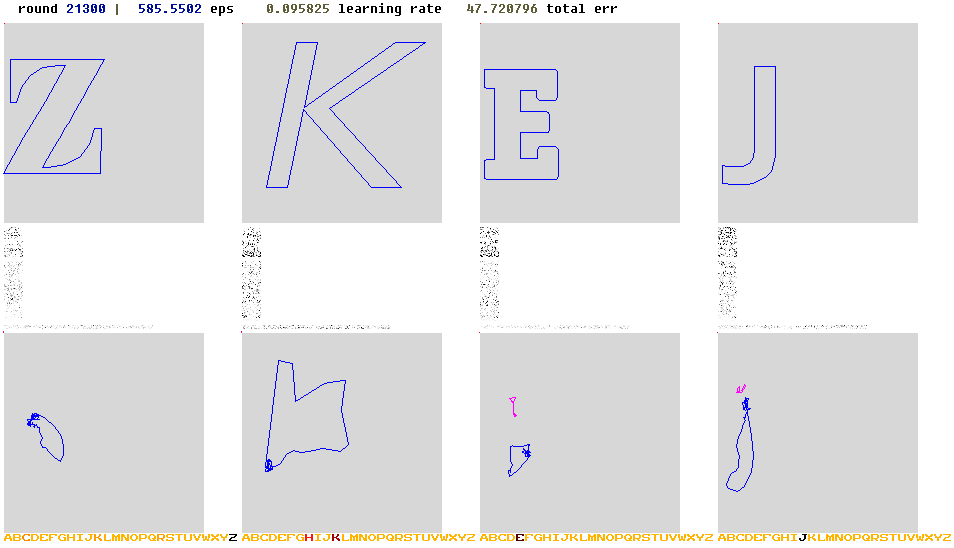
\includegraphics[width=0.9 \linewidth]{trainingvector}
\caption{ Screenshot of {\tt train.exe} running on the first vector-based
  version of the problem. Shown is the \makelowercase\ model's output
  (bottom) on four shapes from four fonts (top). Some dust in between
  is the activation of the network's layers. At the very bottom, the
  26 predictions for ``what letter is this?''. The output for
  \letterform{j} is not too bad; you can see the distinct dot (a
  separate contour) and it sort of looks like a \letterform{j}. The
  \letterform{e} also has two pieces as expected but is otherwise
  garbage. The model is unsure whether the second input is an H
  or a K, and has predicted a shape sort of ambiguously between those
  two. The \letterform{z} is also an embarrassment.
} \label{fig:trainingvector}
\end{figure}

I was so {\tiny confident} that this wouldn't work that I only trained
a \makelowercase\ model and didn't even worry about the more
complicated simultaneous training setup yet. I ran this for about
22,000 rounds, some 90 million training examples. Indeed it does not
work (Figure~\ref{fig:trainingvector}). It is not a total catastrophe,
though. We can tell from the 26 bonus outputs that the model can
clearly recognize letters (though perhaps just by memorization). Some
of the shapes it generates are along the right lines. ({\em Along the
  right lines}, get it??) I did not feel ANGRY at these results
because I expected it to not really work. Still, it ``has output'' and
so it can be used to generate a font. I made every glyph in Comic Sans
MS~\cite{comicsans} lowercase using the model (with the exception of the
\letterform{{\sf \%}} character, which has too many contours---{\it five}!).
Mostly this model produces small, non-confident scrawls, like little
grains of sand, so this font is called {\bf Comic Sands}
(Figure~\ref{fig:comicsands}). The TrueType version can be downloaded
from my website and installed for your desktop publishing
needs.\footnote{Font downloads are available at
  \url{http://tom7.org/lowercase/}.}

\begin{figure*}[tp]
\centering
  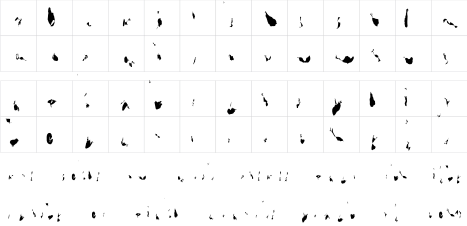
\includegraphics[width=0.95 \linewidth]{comicsands}
\caption{
  Type specimen for the generated font {\bf Comic Sands}. This is
  the hateful Comic Sans MS run through an early vector-based lowercasing
  model (Section~\ref{sec:vectorversion}). At top are Comic Sans's letterforms
  \letterform{A}--\letterform{Z} run through the model and so ``made
  lowercase'' (it's obviously garbage). Next are
  \letterform{a}--\letterform{z},
  made even more lowercase. Also rubbish.
  At the bottom are the illegible pangrams
  ``Dr.~Jock, TV Quiz Ph.D., bags few lynx''
  and ``Sphinx of black quartz, judge my vow!'' Although the output
  barely resembles letters, it does have a certain wispy
  Rorschach aesthetic, like a collection of delicate moths pinned
  to paperboard, that one could consider framing or publishing in
  the proceedings of SIGBOVIK 2021. It is certainly an improvement on
  the original font.
} \label{fig:comicsands}
\end{figure*}


\subsection{Just try making it more complicated!} \label{sec:complicated}

This problem of predicting the vector shape directly is a lot to ask
of a neural network, at least set up this way. One thing that did not
sit well with me is that the network could in principle generate a
perfect-looking result, but because it didn't have the points in the
expected order, it would be penalized. This makes it harder to learn,
and more prone to overfitting.\footnote{For example, imagine if the database
contains two versions of Helvetica that just have their points in a
different order---which is very likely the case btw---the model will
have to learn how to distinguish between these, but using information
we just don't care about.} This was one case where my questionable
reflex to make things more complicated did pay off!

First, I reduced the number of points in the input and output.
Reducing the dimension of the function being learned generally makes
learning a lot faster. This had the side-effect of reducing the number
of eligible fonts (by about half), and by nature these fonts are
simpler shapes. These effects alone could be responsible for the
improved performance of this second try.

I also output each contour's points in a normalized order, starting
from the point closest to the origin. This removes one needless degree
of freedom.\footnote{We can see (well, it's not pictured since I have
  far exceeded a reasonable number of figures in this paper, but {\em
    I} can see) how this manifests in the biases on the output layer,
  which are a proxy for the ``average prediction''. In the first
  model, because of the unstructured order, these are mostly near 0.5
  (center of the character) or 0.0 (degenerate, unused contours). In
  this new model, the distribution of biases is much more flat; it can
  learn that ``the first point tends to be near 0.25,0.25'' and ``the
  seventh point tends to be near 0.64,0.3.''}

Aside from the changes in the input (now 254 nodes) and output (280),
this second version has three sparse hidden layers of size 508, 508,
and 560 nodes; the first two are dense and the latter sparse. The
final model after some pruning had 609k parameters.

As this was training, I worked on another improvement. Ideally we
would compute the difference between the predicted shape and the
expected shape, regardless of how they're drawn. Aside from being a
bit computationally challenging, this won't really work because we
need to attribute error directly to each output in order to actually
update the model in training. I spent a valuable vacation day writing
a routine to compute the best alignment of points between the actual
and expected outputs (Figure~\ref{fig:trainingrotate}). Aside from being
harder than it looked, my alignment code ended up being pretty slow
relative to the rest of training, even worse since it ran on the CPU
instead of GPU, which reduced the training speed by $50\%$. I let it
run for 80,000 rounds, some 331 million training examples, but
eventually got bored of waiting on this approach that was slow to
train and seemed like a complicated version of an bad, oversimplified
approach. So, I control-C'd that thing and threw this whole endeavour
in the trash! But I must have confused the Recycle~Bin icon with the
fairly complicated export-to-TrueType Font process that I built,
because I ran the model on the venerable Futura~\cite{futura} font and
generated {\bf Futurda} (Figure~\ref{fig:futurda}).
%
% \begin{figure}[ht]
% \centering
%   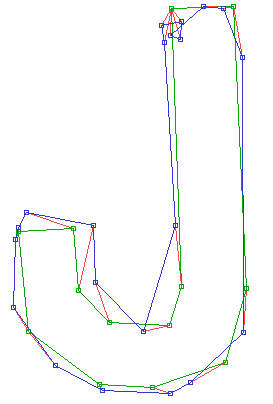
\includegraphics[width=0.5 \linewidth]{rotatej}
% \caption{ Example alignment (from debug UI) of predicted shape (blue)
%   to expected shape (green). We require each point to be mapped (red)
%   to a point from the expected contour in a monotonic order (but
%   several can be mapped to the same one), so that we can attribute
%   error to each point. I hope it was fun to write this code because
%   it was too slow to do pretty much anything but generate this figure!
% } \label{fig:rotatej}
% \end{figure}
%

\begin{figure}[ht]
\centering
  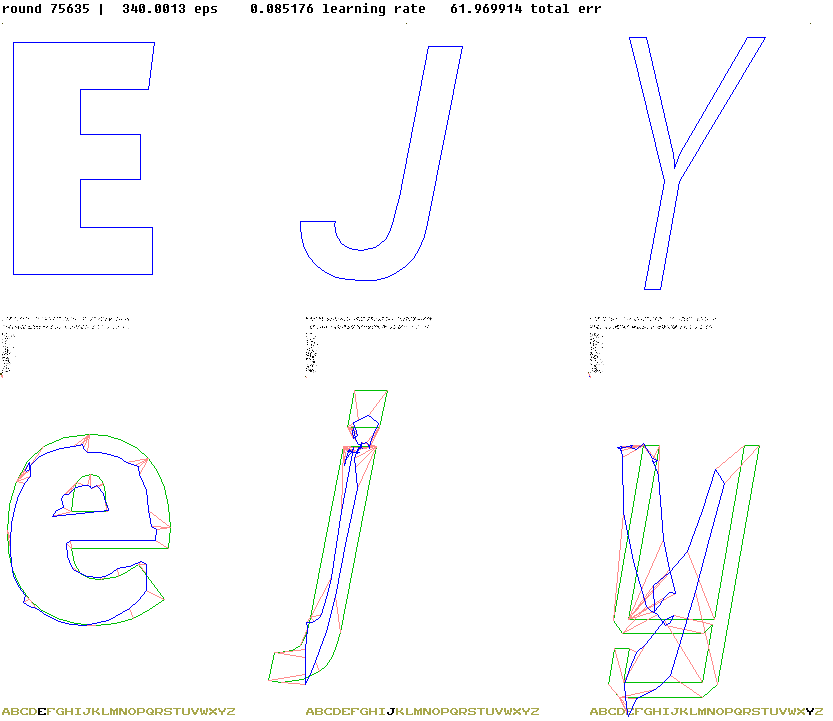
\includegraphics[width=0.95 \linewidth]{trainingrotate}
\caption{ Screenshot (somewhat compacted) of training from near the
  final round of the vector model's training, illustrating the
  permissive loss function that finds the best alignment. At the bottom are
  the predicted lowercase shapes (blue), also shown with their
  expected shape (green). We require each point to be mapped (red)
  to a point from the expected contour in a monotonic order (but
  several can be mapped to the same one), so that we can attribute
  error to each point.
} \label{fig:trainingrotate}
\end{figure}

% XXX downloadable

\begin{figure*}[tp]
\centering
  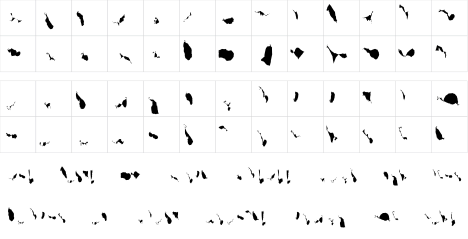
\includegraphics[width=0.95 \linewidth]{futurda}
\caption{ Type specimen for the generated font {\bf Futurda}. This is
  the classic font Futura, run through the final, improved
  vector-based model (Section~\ref{sec:complicated}) to make each
  letter lowercase. The letterforms \letterform{A}--\letterform{Z}
  (top) become quite readable lowercase versions. The extra-lowercase
  \letterform{a}--\letterform{z} are also almost legible, but are
  mostly just scaled-down and screwed up versions of the lowercase
  letterforms. Could definitely imagine this appearing in the
  ``distressed fonts'' category of a 10001 Free TrueType Fonts CD-ROM
  in the 1990s, though.
} \label{fig:futurda}
\end{figure*}

% lowerercase Franklin Gothic. Franklin mint... not guaranteed
% to go up in value


% obviously, need to express different cases of anger at various
% problems or successes?

% the sdf problem

\section{SDFs}

Don't give up! The fixed-size input/output of neural networks is
better suited to something like an array of pixels, and fonts can of
course be represented this way as well. To stay in the realm of what
my desktop computer with a single GeForce 1080 can do, I wanted to
keep the number of inputs and outputs pretty small. There's already an
excellent technique for representing font data as compact bitmaps,
which comes from computer graphics, called Signed Distance Fields
(SDFs)~\cite{green2007improved}. In a standard rasterization of a
font, each pixel of a bitmap contains 1 or 0, or perhaps an
anti-aliased value in-between. In an SDF, the bitmap instead contains
the distance to the nearest edge, and is signed (e.g.~values inside
the shape are $> 0$, value outside are $< 0$). Actually in
practice we offset and saturate the values so that they are all in
$[0,1]$ (or bytes in $[0,255]$), with some nonzero ``on-edge value''
(say, 0.5) standing for ``distance 0''. In order to display the font
at the size of your choice, you then resize the SDF image with bilinear
interpolation, and then simply threshold the image. This works
surprisingly well (Figure~\ref{fig:sdf}).

\begin{figure}[ht]
\centering
  
\includegraphics[width=0.95 \linewidth]{sdf-figure}
\caption{
  The signed distance function representation of a letterform.
  At the very left, a $36\times 36$ pixel rasterization of
  the character without anti-aliasing, for comparison. Any
  scaling of this will have chunky pixel artifacts. Next,
  a $36\times 36$ pixel SDF of same. Third, simply scaling
  that $36\times 36$ image to $180 \times 180$ pixels with
  bilinear sampling. Finally, that image thresholded to
  produce a $180 \times 180$ pixel rasterization, which is
  far superior despite being derived from a $36 \times 36$ pixel
  image. Typically this process is performed at an even higher
  scale and then downsampled to produce an anti-aliased image.
} \label{fig:sdf}
\end{figure}

SDFs seem well-suited for machine learning. They contain more
information per pixel than a plain bitmap, so we can use a smaller
input and output size. On the input side, extremal pixels that would
almost never be set in a bitmap still have significant information
(distance to the character). The error function is just pixel-by-pixel
difference. The rendering of the output is inherently tolerant of some
noise because of the sampling and thresholding. So, this seemed like
it might work really well! (It doesn't work that well.)

I computed some stats on the font database, and determined the
following parameters for the fixed-size SDFs we train on. The images
are $36 \times 36$ pixels. The character box is placed such that there
are $2$ pixels of top padding, and $9$ pixels of left and bottom
padding. The character box is only ``nominal'' in the sense that the
font's contours can exceed its bounds, and this is completely normal
for a letter like \letterform{j} (which goes below the baseline and
often hangs to the left of the origin as well). I used an ``on-edge
value'' of 0.862 (because much more of the SDF is outside the letter
than inside) and the distance is scaled as 0.059 units per pixel
(chosen so that pixels on the outer edge often have non-zero values).
Compared to the first version, I was somewhat more permissive in what
fonts I trained on, since there was no inherent limit to the number of
contours or their complexity. I did exclude fonts whose rasterizations
exceeded the bounds of the SDF, which is possible (very wide
\letterform{W} or low-descending \letterform{j} perhaps) but rare.

\section{The care and feeding of sparse matrices} \label{sec:neural}

Having committed to the representation, again it is ``just'' a matter
of heating up the GPU to apply some linear and non-linear transforms.
The initial network had an input size of $36 \times 36 = 1296$ for the
SDF, and the output the same plus $26$ bonus outputs (one for each
letter, as before). I started with three hidden layers of $1296$, $1296$,
and $2916$ nodes, each sparse ($80\%$ of the weights are zero). Again,
don't take notes. This one works a bit better than before, but still
not impressive. The node references are assigned spatially (something
like the $20\%$ of the nodes on the previous layer that are closest to
the next layer's node) but due to a bug the spatial locality is
actually pretty strange.
% XXX if I show layer weights, forward-reference them here:
% It's responsible for the XXX
Every layer's transfer function is ``leaky relu'' again. It would
definitely make sense to use convolutional layers for this problem, as
features like serifs, lines, curves, and so on could appear throughout
the input and output. I just haven't built support for that in my
weird home-grown software, yet.

I also adapted my weird home-grown software to train the
\makeuppercase\ and \makelowercase\ models simultanously. Two models
fit easily in GPU memory, with plenty of space for a stream of
training data (one training instance is only about 10kb). The only
challenging thing is arranging for them to feed each other generated
``inversion'' examples (Figure~\ref{fig:cotraining}), but this is just
a matter of programming, thank god. I should remember to do projects
that are mostly a matter of programming. Each round, $25\%$ of the
batch consists of inverted examples from the symmetric model's output
from a recent round. Training happens asynchronously, but I make sure
that one model is not allowed to get more than 2 rounds ahead of the
other, because I want this feedback loop to be somewhat tight.

So I did that and let it run for a month. Actually I had to start over
several times with different parameters and initialization weights
because it would get stuck (Figure~\ref{fig:nans}) right away or as
soon as I looked away from the computer. I prayed to the dark wizard
of hyperparameter tuning until he smiled upon my initial conditions,
knowing that somewhere he was adding another tick-mark next to my name
in a tidy but ultimately terrifying Moleskine notebook that he bought
on a whim in the Norman Y.~Mineta San Jose International Airport on a
business trip, and still feels was overpriced for what it is.

\begin{figure}[ht]
\centering
  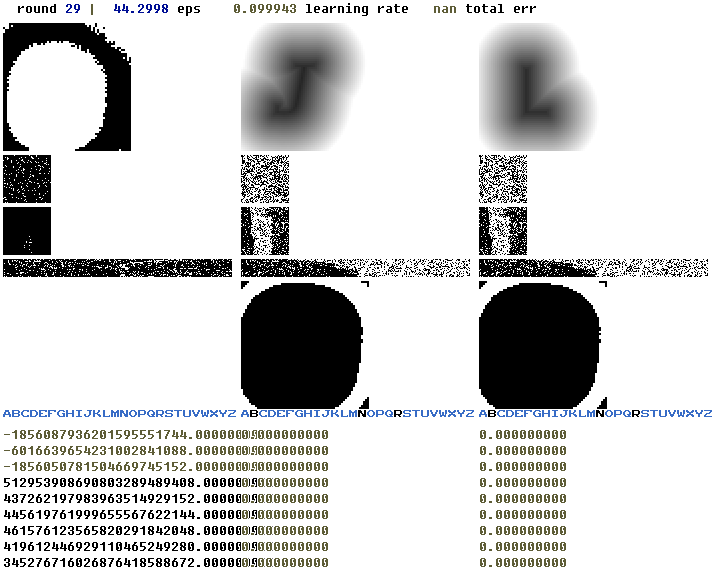
\includegraphics[width=0.9 \linewidth]{nans}
\caption{ Divergent training after only 29 rounds. We have \nan{}
  total error (hard to say if that's good or bad?). The example in
  column one is an inversion example generated by the
  \makeuppercase\ model, which is why it also looks like the Tunguska
  event, just of the opposite sign. The other two are regular inputs,
  whose predicted outputs are black holes. Start over!
} \label{fig:nans}
\end{figure}


\subsection{Fiddly bits} \label{sec:fiddly}
The training error over time appears in
Figure~\ref{fig:sdfmergederror}. It looks like the ones I have seen in
machine learning papers, although I don't like to read other people's
papers because it just seems like spoilers, and reading is the
opposite of writing! There are several noticeable events in the curve,
which came from me fiddling with the parameters or network as it ran.
Here are some of the things I did:

\paragraph{Vacuuming and culling.} Sometimes a node will just be
dead (basically never activates) or an edge weight will be nearly
zero. In these cases an equivalent, tidier network can be made by
dropping the node or edge. Periodically I would perform these
processes, sometimes feeling particularly choppy and removing like
10\% of the parameters at a time. If these parameters are truly
useless with no hope of recovery, we simply get faster training
because there's less work to do. Speed is exhilarating!

\paragraph{Widening.} The opposite thing is to introduce new nodes.
Adding nodes to hidden layers is pretty easy. The thing that worked
best for me is to increase the size of the layer by 10--15\%, where
each new node has random incoming weights and bias 0. Then for each
node on the next layer, I add edges to some subset of these new nodes
(again generally 10\% of them) with weight 0. Since this weight is
zero, the network computes the same function, but has new gradients
to explore (in practice, it then experiences some shock after a
few training rounds, but then quickly fine-tunes this away). More
parameters means slower training, but also more potential to learn
interesting functions, or overfit! Danger is exciting!

\paragraph{Deepening.} It's also possible to add layers once the
network is trained. This can be done anywhere, but I liked doing it on
the output layer because this gets the most direct feedback from the
training examples, and so it updates quickly and changes there are
easy to understand. If you append the identity matrix (new layer is
the same size as the previous; each node has weight 1.0 to its
corresponding node and 0.0 elsewhere) then this network computes
the same function but has new gradients to explore. Adding a layer
did seem to help unlock a new training regime
(Figure~\ref{fig:sdfmergederror}); subjectively it also reduced
some weird artifacts in the SDFs that the model used to predict (makes
sense; this most natural thing for this layer to do is learn how to
predict a ``correction'' from the old prediction, for example
by smoothing/sharpening it). This seems to be borne out by the
weights, which are also fun to look at (Figure~\ref{fig:lastlayer}).
All problems in computer science can be solved by an additional
layer of indirection!

\paragraph{Generating features.} On the other side, randomly sampling
pixels from the input SDF does work, but I superstitiously believed
that it might be better to have more spatially meaningful features. I
wrote a program to generate a bunch of random simple features (one
line/blob with positive weights, one line/blob with negative weights).
It then chooses a set of them that are both {\em good} (maximum
standard deviation on a sample of training data) and {\em different
  from one another} (redundant or even partially redundant features
are less valuable). It was nice to satisfy my supersition, and the
dark wizard of superstitious fiddling with neural networks in the
hope that they do the thing was pleased as well. The features are
at least handsome (Figure~\ref{fig:makefeatures}). Creativity is
enriching!

I presume these are all standard things that neural people do, but they
do better and smarter versions of them because they are willing to
read other people's papers instead of trying to figure things out from
scratch all the time. But you gotta occupy yourself somehow while it
crunches for a month.


\begin{figure}[ht]
\centering
  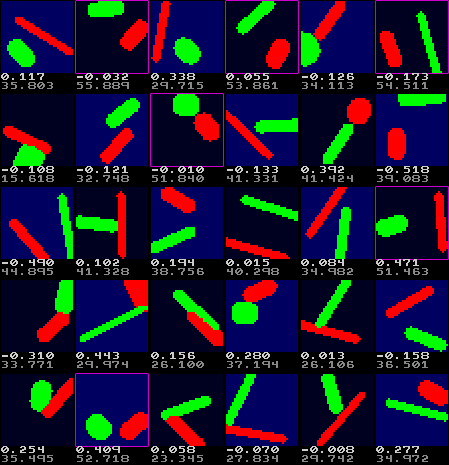
\includegraphics[width=0.99 \linewidth]{makefeatures}
  \caption{ Some randomly-generated features with the selected ones
    outlined in magenta, mostly shown here for aesthetic reasons.
    Savvy Twitter user {\tt @iotathisworld} sees this as ``the classic
    question: machine vision classification or 90s roller rink carpet
    pattern?'' to which I deflect: ``Sorry, it's actually modern day
    Port Authority bus upholstery or Gram stain of same!'' (But
    actually machine vision classification was basically correct.)
  } \label{fig:makefeatures}
\end{figure}


\begin{figure}[ht]
\centering
  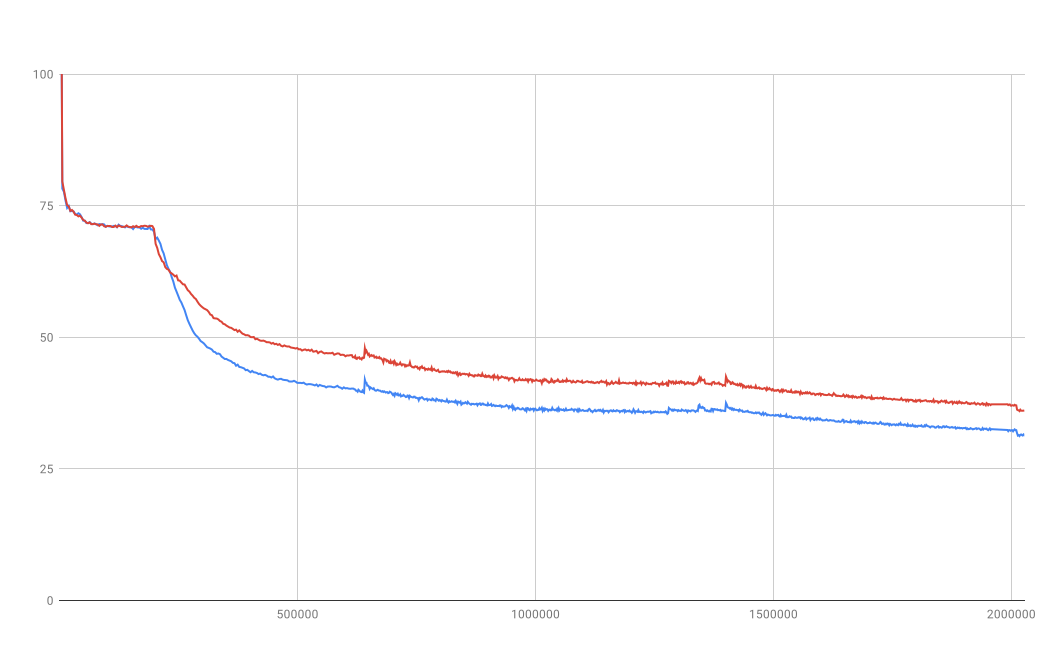
\includegraphics[width=0.99 \linewidth]{sdfmergederror}
\caption{ The training error for the SDF models. The red curve is the
  \makeuppercase\ model, which generally has a higher error rate
  (perhaps simply because uppercase letters usually have more pixels
  set) and blue is \makelowercase. The first few rounds have error
  that's off the charts, well above 100. The most dramatic event is
  around round 200,000, where I reduced the weight decay factor to
  $0.999995$ (from $0.9995$). I guess you just need more nines to be
  more reliable. There are some other visible peaks, which occur when
  I do things like remove nodes with very low weights or which are
  almost never activated (Section~\ref{sec:fiddly}). These momentarily
  increase error but it is easily fine-tuned away (e.g.~by learning
  new biases). The peak at around 1.4M rounds is when I added a new
  layer to the end of the model, which does seem to create a new
  training regime (clear downward slope now); but this also
  significantly increases the training cost per round. Even after
  2,000,000 rounds, the network is still apparently improving, but at
  a speed of about 1 pixel loss per several weeks. Eventually the
  extremely strict SIGBOVIK deadlines mean you just have to call it done.
} \label{fig:sdfmergederror}
\end{figure}


\begin{figure}[ht]
\centering
  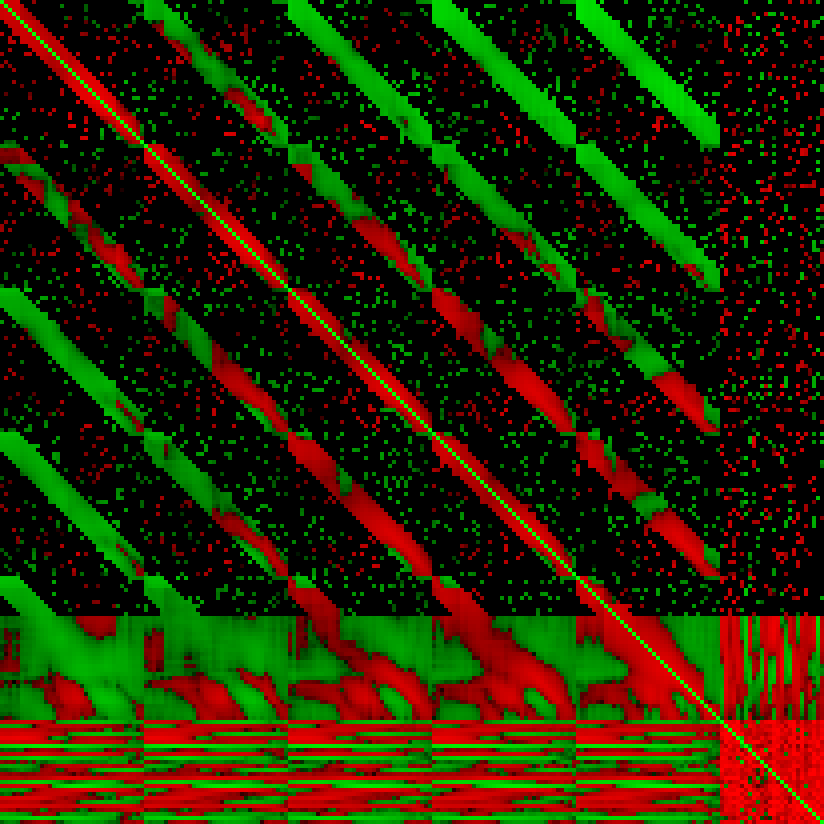
\includegraphics[width=0.99 \linewidth]{lastlayer}
  \caption{ The bottom-right corner of the weight matrix for the final
    layer of the network. This layer was added to the network after
    1.36 million rounds, initially as the identity matrix, and so can
    be thought of partly as a correction of the network's output prior
    to that round (though the remainder of the network continues to
    evolve). The x-axis is the output nodes, and the y-axis is the
    nodes of the previous layer. Note for example that the last 26
    columns look pretty different; these are the predictors for the 26
    letters, which occur in the output after the SDF pixels. Green
    means positive and red means negative, so if you are looking at
    this in a black-and-white printout, that may explain your current
    confusion. The exact diagonal is a strong green, close to 1.0,
    although over time these weights do diverge from the identity
    somewhat. In the bottom-right corner of size $26^2$, we are
    looking at how the 26 letter predictors are derived from the
    previous layer's predictions. We see that most letters are
    negatively correlated (makes sense; only one will ever be 1.0)
    although there are some oddities (probably because it found some
    other, better correlates). Nodes on this new layer have dense
    references to these 26 predictions on the previous; this means
    that the bottom row kind of represents biases for each of the 26
    letters (what does an average 'e' look like?). I also included a
    dense region above that, but this appears to have simply evolved
    the same way as other $36^2$ chunks have (the rest are sparse).
    These chunks have a large amount of spatial similarity (suggesting
    that the sparse sampling would be adequate), with a meaning like
    ``if this area of the image is bright, then this pixel should
    be less bright.'' It is interesting that the pixels immediately
    next to the diagonal are almost always strongly negative
    (sharpening operation). ``Thank you for attending my TED talk.''
    ---\,Figure~\ref{fig:lastlayer}}
  \label{fig:lastlayer}
\end{figure}

For completeness, some other innovations that I feel are worth
mentioning:

Making the GPU code faster has really high value (could save weeks of
waiting). Since I am using OpenCL (whoa, yeah, stop me right there, I
know) I found a good technique was to generate different OpenCL code with
constants baked for each layer (for example their size and
\verb+indices_per_node+); this allows the compiler to use faster
tricks in inner loops for e.g.~multiplication by a compile-time constant
instead of depending on an argument or data. I have different routines
for sparse and dense layers. It might even make sense to recompile the
kernels for other parameters that change over the lifetime of
training, like the learning rate. The {\tt fma} instruction (so named
for the physical law $F=MA$) is a bit faster than
\verb|potential += w * v|, and I guess the compiler can't do this
itself because of IEEE horrors. But like, who cares? In my opinion you
should be able to put it in ``fast machine learning mode'' where it
readily makes precision errors, with a command-line option like
\verb+--fml+. With all the tweaking, the easiest win was to use the
{\tt restrict} keyword on arguments to tell the compiler that the
input cannot alias the output, for example; this presumably helps
it schedule instructions better.

Various things in training run in parallel threads (e.g.~processing
fonts, but also moving data to the GPU, backpropagation for each
example, etc.). For a long time I had just been explicitly setting
parallelism using superstitious constants. For this project I finally
just wrote something that would automatically and empirically
determine the number of threads that yielded the highest throughput,
and persisted that information across program starts. This was a
good idea and enters the permanent rotation.

The actual error on the predicted SDFs is pretty low; for the
\makelowercase\ model it is around 31.3, which is like if 2.4\% of the
pixels were (completely) wrong, but the rest is exactly correct. In
reality, of course, the error is distributed throughout the pixels,
and some errors are a lot more important than others. Particularly,
near the threshold value, a pixel goes from from being considered ``in
the letter'' to ``outside'' with tiny changes in its value. Changes to
a pixel with a value near 0.0 or 1.0 usually doesn't affect the output
shape at all, in contrast. So one thing I did was map the loss
function (comparing expected pixel value to actual) to ``stretch out''
the region near the threshold, increasing the penalty (basically, the
derivative) in that region and decreasing it elsewhere. Looking at the
code again right now, I realize that I only applied this to the first
row of the SDF (\verb+idx < SDF_SIZE+ instead of
\verb+SDF_SIZE * SDF_SIZE+), so that was dumb AND MAKES ME {\bf
  ANGRY}. I will say in my defense that at least I felt disappointed
at the time that it didn't seem to make a difference! (The dark
wizard of superstitious fiddling nods sagely.

% you propagate my back, I'll propagate yours

Ultimately, each of the two models was trained for over 2 million
rounds, which corresponds to 510 million training examples. Each
model is about 24 megabytes.

\subsection{Upperercase and Lowerercase fonts} \label{sec:fonts}

Now that we have these expensive models, we can use them to make
arbitrary letterforms uppercase or lowercase. The output is readily
rasterized (using the standard thresholding approach for SDFs) but
we'd actually like to have vector representations so that we can
use them as TrueType fonts for our desktop publishing needs.

\subsection{Tracing}
Automatically tracing bitmaps into vector form is no doubt a solved
problem, but I chose not to look at spoilers. Since we actually have a
signed distance field, we can build a tracing routine directly off of
that. The approach I took consists of three steps. First, I generate a
bitmap of the SDF (at its native size) using the threshold. I separate
the image into a nested tree of connected components in this pixel
space; each component knows its single parent and whether it is
``land'' (inside the shape) or ``sea''. Characters like \letterform{e}
need internal cutouts, which are represented by a different winding
order (clockwise or counter-clockwise) for the contour. Some of the
tricky cases in computing this tree structure are given in
Figure~\ref{fig:connected}. Once I have this tree structure, I trace
each pixel mass recursively (Figure~\ref{fig:trace}). I find a pixel
on the edge, and then walk around that edge clockwise (simple case
analysis on the three pixels ahead of me). As I walk the edge, I look
at the normal (orthographic as we are doing orthography) of the edge
and see where it reaches the edge value on the SDF; this point (a
float) is output into the contour. The process is guaranteed to return
to where we started. I recurse by negating the SDF (outside
becomes inside) and bitmap (land becomes sea), and reverse the winding
order of the result of recursion.

This gives me a perfectly fine line-based outline of the SDF's shape.
Since I output points at every pixel, sometimes these points are
inefficient (e.g.~a series of colinear points on a straight line),
and sometimes they reflect sharp corners that are not aesthetic. So
I then take a second pass at each contour, and try fitting B\'ezier
curves to sequences of points while the error remains low. Again I
did fitting with a black-box optimizer, which is nice. However,
the function being minimized also needs to be able to find the
closest point on a B\'ezier curve to another point, and although
this can also be done easily with the black-box optimizer, nesting
an optimizer invocation inside another one proved to be way too slow.
I found an old algorithm in a book I owned and was stymied by as a
child~\cite{glassner1990graphics}.

\begin{figure}[ht]
  \centering
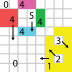
\includegraphics[width=0.6 \linewidth]{connected}
\caption{
  Some tricky cases to think about when generating the nested
  connected components, as the first step of tracing SDFs. Area
  {\bf 0} is the outside of the entire letterform, but note that
  we should include the top-left corner even though it is not
  reachable without leaving the bounds of the image. Area {\bf 1}'s
  parent is 0; it has two holes within it, Areas {\bf 2} and {\bf 3}.
  At the top left, the four pixel chunks making up area {\bf 4} are
  not actually connected, but they separate the hole which is
  child are {\bf 5}. This hole must have one parent, so it means
  that all four pixel chunks are part of the same area {\bf 4}.
} \label{fig:connected}
\end{figure}

\begin{figure}[ht]
  \centering
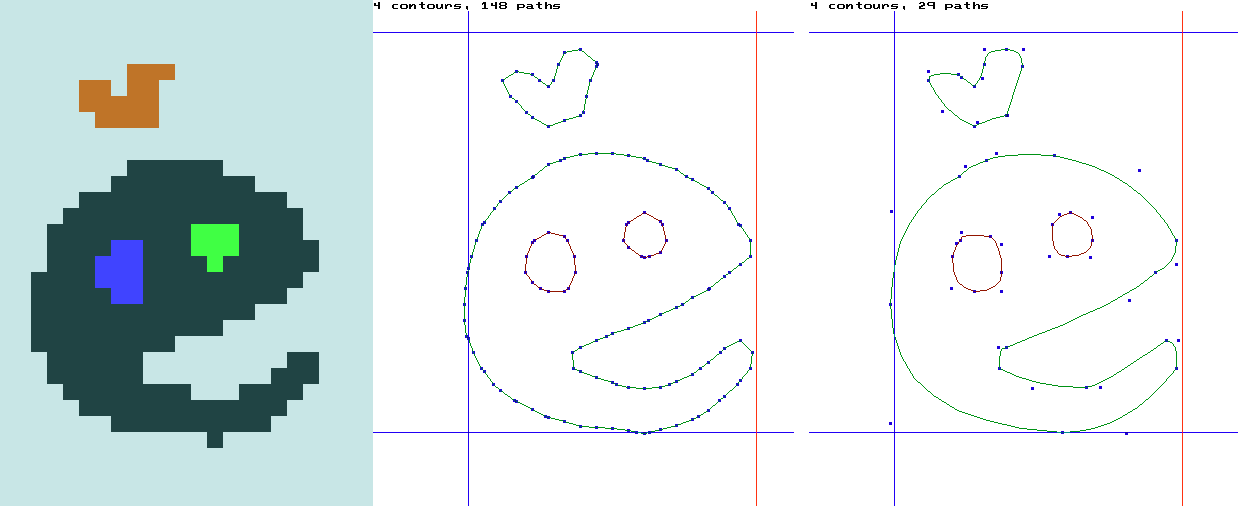
\includegraphics[width=0.95 \linewidth]{trace}
\caption{ Tracing the SDF from Figure~\ref{fig:sdf} into vector
  format. Left image shows the nested connected components. Middle
  image is the initial straight-line trace, and the right image
  shows the simplified contours using quadratic B\'eziers.
} \label{fig:trace}
\end{figure}


\begin{figure*}[tp]
\centering
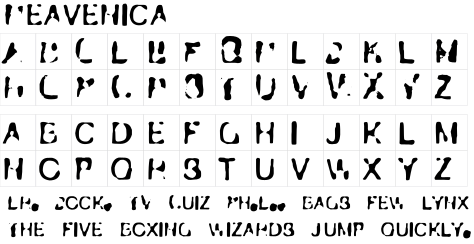
\includegraphics[width=0.9 \linewidth]{heavenica} \\[0.5in]
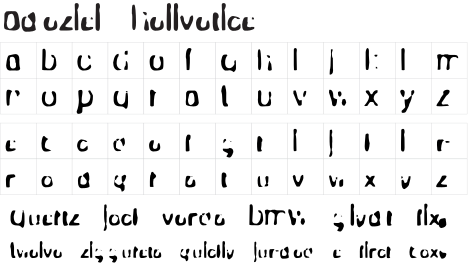
\includegraphics[width=0.9 \linewidth]{spezialhellvetica} \\
\caption{
  Type specimens for the generated font {\bf Heavenica} (top)
  and {\bf Spezial Hellvetica} (bottom). The uppercase letters
  in Heavenica are \makeuppercase\ applied to uppercase letters
  from Helvetica, and the lowercase are \makelowercase\ applied
  to those. These lower-upperercase letters resemble regular
  uppercase letters, as they should; this gives you some idea
  of the quality of the model. Spezial Hellvetica is the
  symmetric thing (its lowercase letters are \makelowercase\ 
  of Helvetica's lowercase). The sample text in this latter
  case is ``Quartz jock vends BMW glyph fix. Twelve ziggurats
  quickly jumped a finch box.''
} \label{fig:heavenica}
\end{figure*}

\begin{figure*}[tp]
\centering
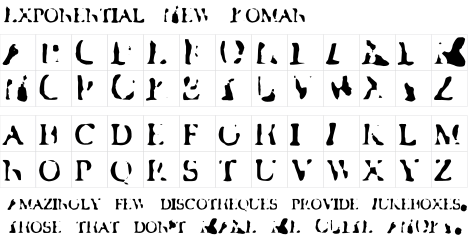
\includegraphics[width=0.9 \linewidth]{expnewroman} \\[0.5in]
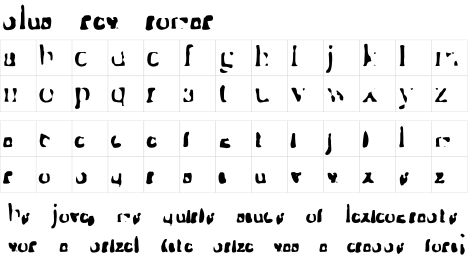
\includegraphics[width=0.9 \linewidth]{plusnewroman} \\
\caption{
  Type specimens for the generated font {\bf Exponential New Roman} (top)
  and {\bf Plus New Roman} (bottom). These were produced with
  the same procedure as in Figure~\ref{fig:heavenica}, but starting
  with Times New Roman. The letterforms are clearly different, so
  it's not as though the models are (just) memorizing a shape for
  each letter. Notably, smudgy serifs reappear when the upperercase letters
  are re-lowercased, as desired.
  Sample text here is ``Amazingly few discotheques provide jukeboxes.
  Those that don't MAKE ME QUITE ANGRY.'' and 
  ``By Jove, my quirky study of lexicography won a prize! (the prize
  was a crappy font)''
} \label{fig:roman}
\end{figure*}


\medskip
Now we're all set up to take an input shape (e.g.~from an existing
font), run the \makeuppercase\ or \makelowercase\ model(s) on it,
maybe multiple times, and trace the resulting SDF into a vector form
that can be used in a font. I did this on the canonical sans serif
font Helvetica~\cite{helvetica} and serif font Times New
Roman~\cite{timesnewroman}.

Helvetica means ``of Hell'', so making the font more uppercase give us
{\bf Heavenica} (Figure~\ref{fig:heavenica}), since Heaven is ``up''
from Hell. What's lower than Hell? Spezial Hell,\footnote{
  I first learned about Spezial Hell from a Rugen Br\"au beer that I
  drank in the Alps in Grindelwald, Switzerland ({\it la
    Conf\'ed\'eration H\'elvetique}).
  % Conf\oe{}deratio Helvetica
}
%
as in ``There's a Spezial Hell for the scalpers and cryptocurrency
environmental terrorists stockpiling GeForce 3000 series cards so that
I can {\em not} just get {\em one} darn card at a reasonable price for
my silly SIGBOVIK experiments.'' So the extra-lowercase version of
Helvetica is {\bf Spezial Hellvetica} (also Figure~\ref{fig:heavenica}).

Times New Roman refers to the multiplication operator in algebra,
which has a natural uppercase in exponentiation. Thus the uppercase
version of Times New Roman is {\bf Exponential New Roman}. Computing
Tetration New Roman or $\uparrow\uparrow\uparrow\uparrow$ New
Roman~\cite{knuth1976coping} is straightforward, but extremely
punctilious SIGBOVIK page limits preclude showing them here. Of course
the lowercase version is {\bf Plus New Roman} (and similarly implies
Successor New Roman). Both fonts are shown in Figure~\ref{fig:roman}.

The vector-based {\bf Futurda} font (Figure~\ref{fig:futurda}) is in
some ways more readable than these, but for the sake of comparison,
note that these fonts are actually doing something more interesting,
as they are built with both the \makeuppercase\ and
\makelowercase\ models. Futurda's \letterform{A}--\letterform{Z} are
just the lowercase of existing uppercase letters, which already has a
correct solution and which a ML model can simply learn through
memorization. In contrast, none of the letterforms in Heavenica can
come through memorization of a training example (at worst, memorizing
an inversion example generated by the other model after {\em it}
memorized something). Subjectively, the fonts are not very readable
and only slightly interesting, but the two models did demonstrate a
reasonable ability to invert one another's behavior.

\section{Perfect letters, hallucinated} \label{sec:hallucination}

Oh, you don't like letters that look {\em bad}? Instead you want
letters that look {\em good}? How about {\em best}?

The fonts in the previous section were created by modifying the case
of existing letterforms, with mixed success. We can also do this to
any letter-like shape. I built a UI for drawing letters and seeing
them uppercased and lowercased (and then re-lowercased and
re-uppercased) live, but it's impossible to demonstrate in paper form.
It's pretty much what you'd expect.

The UI also tells you how much your input resembles the various
existing letters \letterform{A}--\letterform{Z} and
\letterform{a}--\letterform{z} using the 26 bonus outputs that each
model predicts. For example, I learned that the ``Cool
S''~\cite{wikipediacools}:

\begin{center}
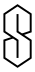
\includegraphics[width=0.1 \linewidth]{cools}
\end{center}

\noindent does not much resemble an S.
% XXX ideally, numbers matching a scene in the video?

This begs us to ask the question: What shapes {\em do} look like
letters? Since the models will tell us, I can just search over shapes
and ask them. The first thing I tried was to just generate random
shapes and optimize their parameters to produce the highest possible
prediction for the target letter, and the lowest possible prediction
for the rest. This preduced results that are fully bonkers
(Figure~\ref{fig:bonkersf}). 

We can improve the results by searching for inputs with a ``perfect''
prediction (1.0) rather than making it as high as possible. These
results may not have been fully bonkers, but were at least downright
wacky. Since there appear to be a large variety of inputs that the
model judges as ``perfect'', the most appealing results from this
excursion involved scoring some additional properties of the
hallucinated inputs to discourage them from being so barmy. I
generated $8 \times 8$ bitmaps, plenty of pixels to make readable
letters on classic computers. Rather than allowing them to be
arbitrarily noisy, I also weakly optimized for (1) the number of
pixels set being close to half (2) minimal transitions between
on and off along each row and column. This produced shapes that
are basically letter-like, but weird (Figure~\ref{fig:perfect}).

\begin{figure}[tp]
\centering
  
\includegraphics[width=0.9 \linewidth]{bonkersf}
\caption{ A randomly generated SDF (left) and its rasterization
  (right) which maximized the predicted score for \letterform{F}
  (1.893 out of a nominal 1.0) while 
  scoring all other letters low. Parts are recognizable as an
  \letterform{F}, but other parts are fully bonkers. This is actually
  one of the least weird ones.
} \label{fig:bonkersf}
\end{figure}

\begin{figure*}[tp]
\centering
  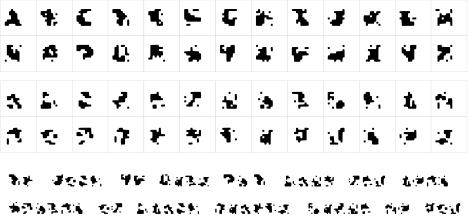
\includegraphics[width=0.9 \linewidth]{perfecthallucination}
\caption{
   Type specimen for the generated font {\bf Perfect Hallucination}.
   Each letter is an 8x8 bitmap that looks as close to ``perfect''
   as possible to the model. Perfect here means that for \letterform{C},
   the \makelowercase\ model outputs as close to the vector
   $[0, 0, 1, 0, 0, \ldots, 0]$ (in its 26 letter predictors; the
   actual lowercasing is ignored) as the optimizer could find. (Of
   course I didn't search all $2^{64}$ inputs, but errors are
   on the order of one part per thousand). The models are completely
   successful at recognizing normal-looking letters as well, but
   it likes these even better.
} \label{fig:perfect}
\end{figure*}

% LSDF


\section{Chess-playing}

\newcommand\deterministic{
  
\includegraphics[height=0.8em]{deterministic}
}
\newcommand\asymmetric{
  
\includegraphics[height=0.8em]{asymmetric}
}


One obvious thing to do with a program that takes an $8 \times 8$
bitmap and produces some kind of score for it is to use that
program to play chess~\cite{murphy2019blind}. Here I entered
26 such programs in the Elo World tournament~\cite{murphy2019eloworld},
which allows us to see how they perform against each other
and benchmark algorithms. (Badly.)

At each turn, the algorithm takes the board state that would
result from each legal move, and interprets it as an $8 \times 8$
bitmap. It renders that bitmap as an SDF and then runs the
\makelowercase\ model on it, and chooses the move that minimizes
the difference between its letter predictions and the
$[0, 0, \ldots 1, \ldots 0]$ vector corresponding to the letter
we are ``playing as.'' \deterministic \asymmetric

After tens of thousands of games each, it is clear that the letter-based
players are all bad at chess. Letters \letterform{E} and
\letterform{S} perform the worst (agreed on \letterform{S} being the
worst, thank you very much!), even worse than the ``No, I insist!''
strategy that tries to force its opponent to capture its pieces.
Letters \letterform{K} and \letterform{T} (eponymous! yeah!) perform
the best, but still worse than random. The numeric players like $\pi$
and $e$ are categorically better than the alphabetical ones, but this
is not surprising because chess is more of a mathematical game than a
linguistic one (Figure~\ref{fig:chess}).

\begin{figure}[tp]
  \centering
  \chessboard[setfen=B2k4/8/1b2p2n/1b2p1pr/6Pp/4B2P/4q3/4K3 w - - 10 60,showmover=false]
  \caption{
    The letter \letterform{P} (white) loses to the numeric constant
    $\pi$ (black) after 59 nonsensical moves. The \letterform{P}
    player tries to move pieces such that the board looks like a
    letter \letterform{P} (and no other) to the neural network.
    The $\pi$ player uses
    $3 - \pi$ to arithmetically decode the sequence of legal moves
    (sorted alphabetically by PGN). Neither player is concerned with
    chess, really, but the letter-based players are generally bad
    because they are more likely to get stuck in local minima once
    they are basically happy with the shape of the pieces.
    %  1. Na3 g5 2. b3 e6 3. f4 Nc6 4. e4 Be7 5. e5 a6 6. c3 f6 7. h3 Bb4 8. g4 h5 9. Nf3 h4 10. Nd4 Rb8 11. Nf5 Na5 12. Nc2 Rh7 13. Nce3 d6 14. Qf3 Rh5 15. Nh6 Bd7 16. Bc4 c6 17. Rf1 Qc7 18. fxg5 Bxc3 19. b4 Bxb4 20. a3 Bc8 21. axb4 Qe7 22. Kd1 c5 23. d3 Nxh6 24. Ke2 Ra8 25. Rd1 dxe5 26. Bb5 Bd7 27. Ke1 c4 28. Nd5 Qg7 29. Nc3 Nb3 30. Bc6 Nd4 31. Be3 Nc2 32. Kf1 cxd3 33. Rdc1 d2 34. Qf4 Qh7 35. Qd4 Na3 36. Rxa3 a5 37. Qe4 b6 38. bxa5 dxc1=B 39. Qd5 Kd8 40. Qc5 Rb8 41. Ke1 Qe7 42. Bf3 fxg5 43. Bb7 Bxa3 44. Ba6 Bxc5 45. Bb5 Qd6 46. Ba6 Ba4 47. axb6 Bc6 48. Bc8 Qe7 49. Ba6 Rb7 50. Bxb7 Bxb6 51. Na2 Bb5 52. Nc1 Qa3 53. Nd3 Kd7 54. Nb2 Qxb2 55. Bc8 Ke8 56. Ba6 Kd7 57. Bc8 Kd8 58. Bb7 Qg2 59. Ba8 Qe2
    } \label{fig:chess}
\end{figure}

% figure? drop it?
{
  \tiny
\begin{tabular}{lrrrr}
name & elo & win & loss & draw \\
\hline  
worstfish & 395.95 & 10 & 44406 & 18584 \\
no i insist & 605.47 & 0 & 20405 & 42595 \\
letter f & 605.60 & 1341 & 21653 & 40006 \\
letter y & 606.00 & 1347 & 21688 & 39965 \\
letter b & 607.39 & 1705 & 21870 & 39425 \\
letter p & 607.61 & 1790 & 21963 & 39247 \\
letter l & 608.75 & 1370 & 21306 & 40324 \\
letter j & 610.86 & 1737 & 21525 & 39738 \\
letter u & 611.41 & 1363 & 20947 & 40690 \\
letter c & 612.38 & 1264 & 20787 & 40949 \\
huddle & 612.60 & 1172 & 20494 & 41334 \\
letter n & 612.81 & 1395 & 20802 & 40803 \\
letter w & 613.64 & 1342 & 20723 & 40935 \\
letter g & 613.72 & 1339 & 20660 & 41001 \\
letter v & 614.18 & 1390 & 20606 & 41004 \\
letter h & 615.04 & 1328 & 20452 & 41220 \\
letter r & 615.22 & 1826 & 20932 & 40242 \\
letter x & 615.70 & 1414 & 20457 & 41129 \\
letter m & 616.31 & 1774 & 20809 & 40417 \\
letter q & 618.85 & 1378 & 19993 & 41629 \\
letter o & 619.08 & 1502 & 20078 & 41420 \\
letter z & 620.09 & 1745 & 20275 & 40980 \\
letter d & 620.10 & 1730 & 20369 & 40901 \\
letter a & 620.57 & 1819 & 20212 & 40969 \\
letter i & 622.50 & 2169 & 20424 & 40407 \\
letter k & 622.90 & 1755 & 19878 & 41367 \\
letter t & 623.30 & 2237 & 20271 & 40492 \\
\ldots \\
random move & 655.90 & 7267 & 20983 & 34750 \\
\ldots \\
chessmaster.nes lv1 & 1014.74 & 37302 & 13992 & 11706 \\
\ldots \\
stockfish1m & 2831.66 & 60167 & 493 & 2340 \\
\end{tabular}
}

% CAPS LOCK, LOCK, CAPTAIN'S LOCK

% when two letters coincide, a shift-reduce conflict

\section{Other Applications}

People often stop me on the street to ask, Tom, Why did you spend so
much time and energy on this useless SIGBOVIK project? To which I say,
Ha! At least I am not wasting my time {\it reading} SIGBOVIK papers or
talking to strangers on the street! and run off. Although the main
purpose of SIGBOVIK is to confound bibliometrics with ambiguously
good-faith and high-quality research published in a clearly satirical
but superfically decorous venue of a traditionally esteemed university,
it is also possible for such work to have practical applications in
arts and spycraft. You simply need to give it some thought.

For example, it is well known to {\sf internet troIIs} and {\sf DOMAlN
  NAME PHlSHERS} that the uppercase \letterform{i} and loweracse
\letterform{L} are indistinguishable in many fonts, allowing for
various Tomfoolery.\footnote{I actually wrote ``troiis'' and ``domaln
  name phlshers'', hehe!} This can also be used for
steganography---hiding messages inside text---by replacing letters
with their alternates. Each replacement only encodes one bit of
information, however. With the generic ability to uppercase and
lowercase letterforms, we can exploit this ambiguity to generate
a large variety of letterforms that can be used like this.

For example, the following sequence of distinct letters are hard to
distinguish from one another and could all be used in place of a
lowercase \letterform{L} or uppercase \letterform{i}:

\begin{center}
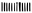
\includegraphics[width=0.25 \textwidth]{stegtaller}
\end{center}

The letterforms are generated by repeated application of the
\makeuppercase\ ($\uparrow$) and \makelowercase\ ($\downarrow$)
networks to the lowercase \letterform{l} from Helvetica. They
are, from left to right: $\letterform{l}$,
$\uparrow \downarrow \letterform{l}$,
$\downarrow\uparrow \uparrow \downarrow \letterform{l}$,
$\uparrow \downarrow\uparrow \downarrow \letterform{l}$,
$\uparrow \uparrow \downarrow\downarrow \letterform{l}$,
$\downarrow\downarrow\uparrow \uparrow \downarrow \letterform{l}$,
$\downarrow\uparrow \uparrow \downarrow\downarrow \letterform{l}$,
$\uparrow \uparrow \uparrow \downarrow\downarrow \letterform{l}$,
$\downarrow\uparrow \downarrow\uparrow \uparrow \downarrow \letterform{l}$,
$\downarrow\uparrow \uparrow \downarrow\uparrow \downarrow \letterform{l}$,
$\downarrow\uparrow \uparrow \uparrow \downarrow\downarrow \letterform{l}$,
$\uparrow \downarrow\downarrow\uparrow \uparrow \downarrow \letterform{l}$.

In this way we can encode much longer bit strings in a single
character, even thousands of iterations deep if there is a reasonable
balance of uppercasing and lowercasing operations. (Too many in a row
will get us stuck; see Section~\ref{sec:lowestcase}.) Not all
sequences lead to a shape like this (commonly they resemble
\letterform{i} or \letterform{L} when starting from \letterform{l}),
but we can easily create a codebook of ones that do. Maybe I have even
hidden an intricate message in this paper for you to discover? (I
didn't.)


% taller:
% adlnotwERTUZ
% 
% shorter:
% ceikmqrsyHQSWXY
% 
% Other applications: Steganography with llIIllIl

% a:
% b: l
% c: ll
% d: ul
% e: lll
% f: lul
% g: ull
% h: uul
% i: llll
% j: llul
% k: lull
% l: luul
% m: ulll
% n: ulul
% o: uull
% p: uuul
% q: lllll
% r: lllul
% s: llull
% t: lluul
% u: lulll
% v: lulul
% w: luull
% x: luuul
% y: ullll
% z: ullul
% A: ulull
% B: uluul
% C: uulll
% D: uulul
% E: uuull
% F: uuuul
% G: llllll
% H: llllul
% I: lllull
% J: llluul
% K: llulll
% L: llulul
% M: lluull
% N: lluuul
% O: lullll
% P: lullul
% Q: lulull
% R: luluul
% S: luulll
% T: luulul
% U: luuull
% V: luuuul
% W: ulllll
% X: ulllul
% Y: ullull
% Z: ulluul

\section{To infinity, but let's stop there} \label{sec:lowestcase}

Wow, this project is pretty involved, huh? Let's just add another
dimension to it!

We looked at what we get when we run \makelowercase\ on an existing
lowercase letter, making it lowerercase. Of course, we can run the
model again, and get an even lowererercase letter. The process can be
repeated indefinitely. As it turns out, lowercasing tends to make
letters smaller and smaller (makes sense) and they eventually just
turn to dust (Figure~\ref{fig:lowestcaseo}) and stay that way (makes
sense; ``dust to dust'').

It's possible to make the results a bit more interesting by injecting
additional energy after each iteration, either by adjusting the gamma
or ``zooming'' into the active area. This seems pretty arbitrary,
though. I think it is right to conclude that the lowestcase versions
of letters are canonically specks of dust.

On the other hand, repeatedly uppercasing produces more interesting
results. Uppercasing usually increases the scale of a letter, but
this effect is limited by the finiteness of the SDF and the fact
that XXX

\begin{figure}[t]
\centering
  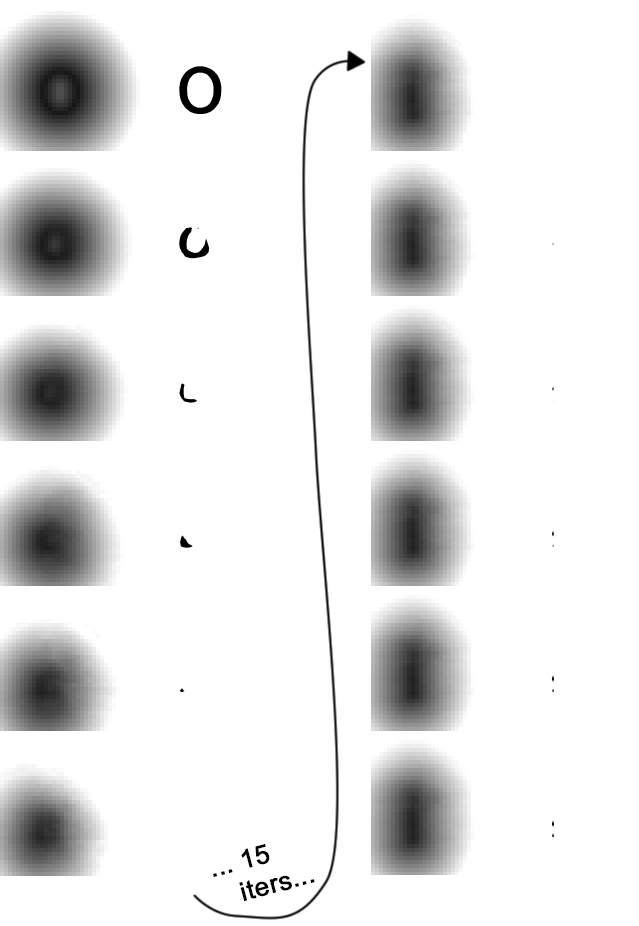
\includegraphics[width=0.80 \linewidth]{lowestcaseo}
  \caption{ The first 27 iterations of the \makelowercase\ model on
    the letter \letterform{o}. The lowercase model generally makes
    letters get smaller and smaller until they disappear. There is
    still energy in the SDF (left column) but no pixels exceed the
    threshold so the rasterization is empty (right column) for about
    16 iterations. Finally it reaches a stable state, a tiny piece of
    colon-shaped dust, easily mistaken for a printing error. All
    letters (from the test font Helvetica) converge to this shape,
    except mysteriously the letter \letterform{v}. Is \letterform{v} a
    different alien species, masquerading as a normal letter for
    millions of years? } \label{fig:lowestcaseo}
\end{figure}


% lowercase uppercase letters etc.
% iterate this a lot of times?
% "to infinity, but let's stop there"

% run it to infinity to see the uppestcase, etc.
% if these vanish, then we have a fixed point.
% if not, or perhaps by doing some auto-gamma, then
% it's like a fractal zoomer, and we can set the
% record on the "most uppercase letter" by running
% a jazillion times.

% lowestcase is just dust, not surprising
% uppestcase is actually a fixed point (not FixedSys)
% ... so it's like a 3D manifold

\begin{figure}[t]
\centering
  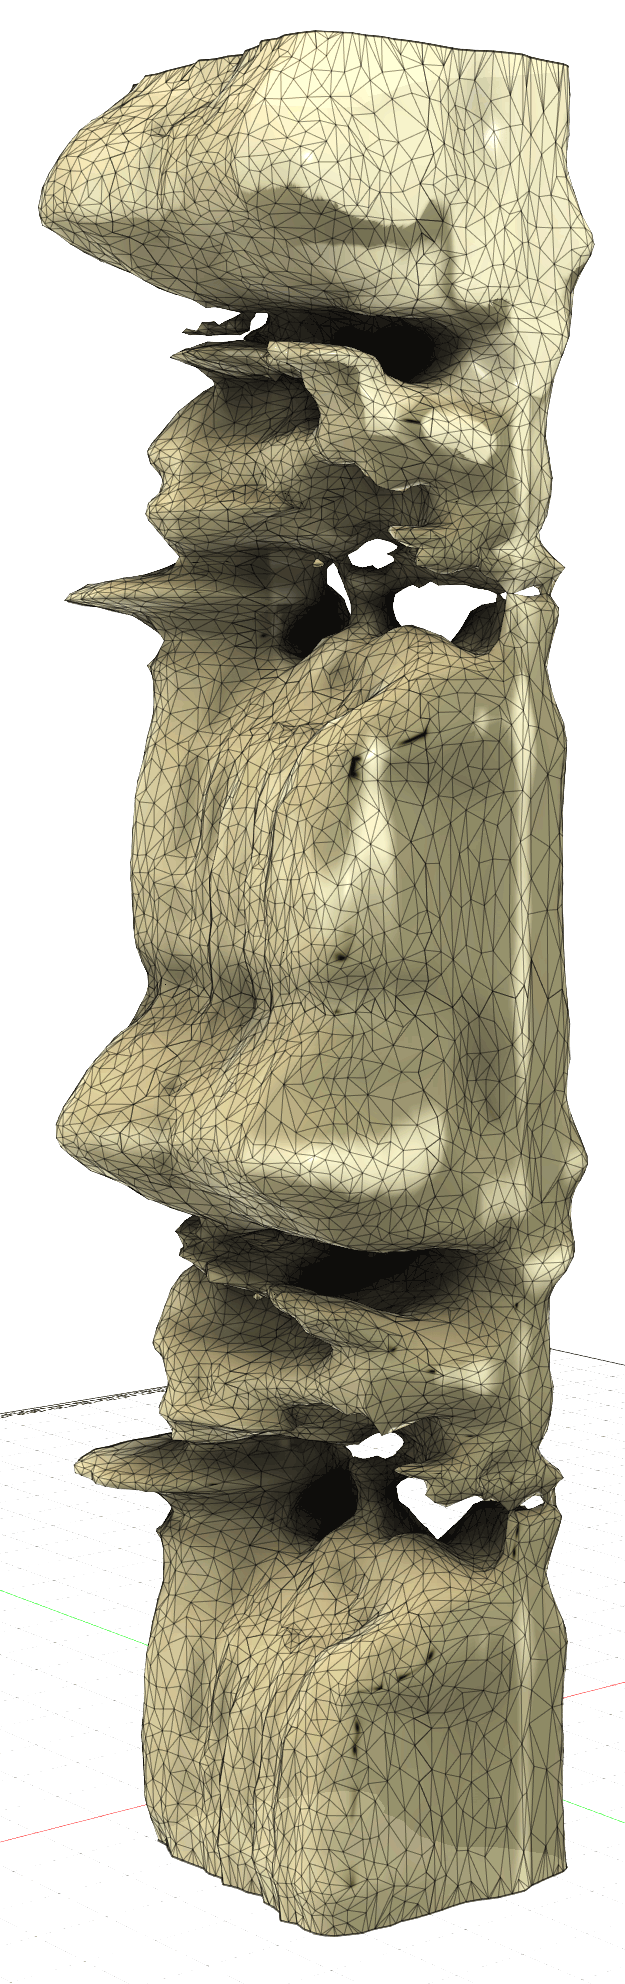
\includegraphics[width=0.7 \linewidth]{uppestcase3d}
\caption{ 3D manifold showing a section of the repeating loop as the
  \makeuppercase\ model iteratively uppercases a letter. (Shown here
  is the input \letterform{q} from iteration 245--377, but they all
  converge to this same periodic shape.) Slices through this shape give a
  letterform's outline (or usually, a linear interpolation between two
  of them). The bottom of the shape is its ``beginning'' but it
  appears to repeat like this forever.
} \label{fig:uppestcase3d}
\end{figure}

% bristol stool chart


\section{Acknowledgements}

For this project I used \verb+stb_truetype.h+ from the excellent stb
collection of single-file libraries~\cite{stb}. I did push its limits
somewhat and ``automatically discovered'' assertion failures and other
crashes (e.g.~during blackbox optimization on all 100k fonts), but it
saved a lot of time. This library only helps with reading the fonts
and generating SDFs. To generate TTFs, I had to write my own pipeline,
which generates FontForge's .SFD (a typo factory right there) files,
and then did the final export with FontForge~\cite{fontforge}. Thanks
Jason Reed for this suggestion, without which I would probably still
be developing my own TTF file writer and custom hinting engine. Finally,
I would like to thank the pseudonymous SIGBOVIK program committee for
overseeing the proceedings, and the \upsigbovik\ program committee
committee for overseeing {\em them}.


\bibliography{lowercase}{}
\bibliographystyle{plain}

\end{document}

